% Copyright (C) 2020 Saurabh Joshi
%% 
\let\negmedspace\undefined
\let\negthickspace\undefined

\documentclass[journal,12pt,twocolumn]{IEEEtran}
%\documentclass[journal,12pt,twocolumn]{IEEEtran}
%
\usepackage{setspace}
\usepackage{gensymb}
%\doublespacing
\singlespacing
%\usepackage{graphicx}
%\usepackage{amssymb}
%\usepackage{relsize}
\usepackage[cmex10]{amsmath}
%\usepackage{amsthm}
%\interdisplaylinepenalty=2500
%\savesymbol{iint}
%\usepackage{txfonts}
%\restoresymbol{TXF}{iint}
%\usepackage{wasysym}
\usepackage{amsthm}
\usepackage{mathrsfs}
\usepackage{txfonts}
\usepackage{stfloats}
\usepackage{cite}
\usepackage{cases}
\usepackage{subfig}
%\usepackage{xtab}
\usepackage{longtable}
\usepackage{multirow}
%\usepackage{algorithm}
%\usepackage{algpseudocode}
\usepackage{enumitem}
\usepackage{mathtools}
\usepackage{tikz}
\usepackage{circuitikz}
\usepackage{verbatim}
\usepackage{hyperref}
\usepackage{chngcntr}
% \counterwithout{figure}{section}
%\usepackage{stmaryrd}
\usepackage{tkz-euclide} % loads  TikZ and tkz-base
%\usetkzobj{all}
\usepackage{listings}
    \usepackage{color}                                            %%
    \usepackage{array}                                            %%
    \usepackage{longtable}                                        %%
    \usepackage{calc}                                             %%
    \usepackage{multirow}                                         %%
    \usepackage{hhline}                                           %%
    \usepackage{ifthen}                                           %%
  %optionally (for landscape tables embedded in another document): %%
    \usepackage{lscape}     
\usepackage{multicol}
\usepackage{chngcntr}
\usepackage{iftex}
%\usepackage[latin9]{inputenc}
\usepackage{geometry}
\usepackage{bm}
%\geometry{verbose,tmargin=2cm,bmargin=3cm,lmargin=1.8cm,rmargin=1.5cm,headheight=2cm,headsep=2cm,footskip=3cm}
\usepackage{array}
\newcolumntype{L}[1]{>{\raggedright\let\newline\\\arraybackslash\hspace{0pt}}m{#1}}
\newcolumntype{C}[1]{>{\centering\let\newline\\\arraybackslash\hspace{0pt}}m{#1}}
\newcolumntype{R}[1]{>{\raggedleft\let\newline\\\arraybackslash\hspace{0pt}}m{#1}}

% \usepackage{graphicx}
%\usepackage{setspace}
%\usepackage{parskip}

\def \hsp {\hspace{3mm}}

\makeatletter

\providecommand{\tabularnewline}{\\}



\makeatother
\ifxetex
\usepackage[T1]{fontenc}
\usepackage{fontspec}
%\setmainfont[ Path = fonts/]{Sanskrit_2003.ttf}
\newfontfamily\nakulafont[Script=Devanagari,AutoFakeBold=2,Path = fonts/]{Nakula}
%\newfontfamily\liberationfont{Liberation Sans Narrow}
%\newfontfamily\liberationsansfont{Liberation Sans}
\fi
\usepackage{tikz}
\usepackage{xcolor}
%\usepackage{enumerate}

%\usepackage{wasysym}
%\newcounter{MYtempeqncnt}
\DeclareMathOperator*{\Res}{Res}
%\renewcommand{\baselinestretch}{2}
\renewcommand\thesection{\arabic{section}}
\renewcommand\thesubsection{\thesection.\arabic{subsection}}
\renewcommand\thesubsubsection{\thesubsection.\arabic{subsubsection}}
\renewcommand\thefigure{\arabic{\thesection}}
\renewcommand\thesectiondis{\arabic{section}}
\renewcommand\thesubsectiondis{\thesectiondis.\arabic{subsection}}
\renewcommand\thesubsubsectiondis{\thesubsectiondis.\arabic{subsubsection}}

% correct bad hyphenation here
\hyphenation{op-tical net-works semi-conduc-tor}
\def\inputGnumericTable{}                                 %%

\lstset{
language=tex,
frame=single, 
breaklines=true
}

%\begin{document}
%


\newtheorem{theorem}{Theorem}[section]
\newtheorem{problem}{Problem}
\newtheorem{proposition}{Proposition}[section]
\newtheorem{lemma}{Lemma}[section]
\newtheorem{corollary}[theorem]{Corollary}
\newtheorem{example}{Example}[section]
\newtheorem{definition}[problem]{Definition}
%\newtheorem{thm}{Theorem}[section] 
%\newtheorem{defn}[thm]{Definition}
%\newtheorem{algorithm}{Algorithm}[section]
%\newtheorem{cor}{Corollary}
\newcommand{\BEQA}{\begin{eqnarray}}
\newcommand{\EEQA}{\end{eqnarray}}
\newcommand{\define}{\stackrel{\triangle}{=}}

\bibliographystyle{IEEEtran}
%\bibliographystyle{ieeetr}


\providecommand{\mbf}{\mathbf}
\providecommand{\pr}[1]{\ensuremath{\Pr\left(#1\right)}}
\providecommand{\qfunc}[1]{\ensuremath{Q\left(#1\right)}}
\providecommand{\sbrak}[1]{\ensuremath{{}\left[#1\right]}}
\providecommand{\lsbrak}[1]{\ensuremath{{}\left[#1\right.}}
\providecommand{\rsbrak}[1]{\ensuremath{{}\left.#1\right]}}
\providecommand{\brak}[1]{\ensuremath{\left(#1\right)}}
\providecommand{\lbrak}[1]{\ensuremath{\left(#1\right.}}
\providecommand{\rbrak}[1]{\ensuremath{\left.#1\right)}}
\providecommand{\cbrak}[1]{\ensuremath{\left\{#1\right\}}}
\providecommand{\lcbrak}[1]{\ensuremath{\left\{#1\right.}}
\providecommand{\rcbrak}[1]{\ensuremath{\left.#1\right\}}}
\theoremstyle{remark}
\newtheorem{rem}{Remark}
\newcommand{\sgn}{\mathop{\mathrm{sgn}}}
\providecommand{\abs}[1]{\left\vert#1\right\vert}
\providecommand{\res}[1]{\Res\displaylimits_{#1}} 
\providecommand{\norm}[1]{\left\lVert#1\right\rVert}
%\providecommand{\norm}[1]{\lVert#1\rVert}
\providecommand{\mtx}[1]{\mathbf{#1}}
\providecommand{\mean}[1]{E\left[ #1 \right]}
\providecommand{\fourier}{\overset{\mathcal{F}}{ \rightleftharpoons}}
%\providecommand{\hilbert}{\overset{\mathcal{H}}{ \rightleftharpoons}}
%\providecommand{\system}{\overset{\mathcal{H}}{ \longleftrightarrow}}
\providecommand{\system}[1]{\overset{\mathcal{#1}}{ \longleftrightarrow}}
\providecommand{\gauss}[2]{\mathcal{N}\ensuremath{\left(#1,#2\right)}}
%
	%\newcommand{\solution}[2]{\textbf{Solution:}{#1}}
\newcommand{\solution}{\noindent \textbf{Solution: }}
\newcommand{\cosec}{\,\text{cosec}\,}
\newcommand{\sinc}{\,\text{sinc}\,}
\newcommand{\rect}{\,\text{rect}\,}
\providecommand{\dec}[2]{\ensuremath{\overset{#1}{\underset{#2}{\gtrless}}}}
\newcommand{\myvec}[1]{\ensuremath{\begin{pmatrix}#1\end{pmatrix}}}
\newcommand{\mydet}[1]{\ensuremath{\begin{vmatrix}#1\end{vmatrix}}}
\newcommand*{\permcomb}[4][0mu]{{{}^{#3}\mkern#1#2_{#4}}}
\newcommand*{\perm}[1][-3mu]{\permcomb[#1]{P}}
\newcommand*{\comb}[1][-1mu]{\permcomb[#1]{C}}
%\numberwithin{equation}{section}
\numberwithin{equation}{section}
%\numberwithin{problem}{section}
%\numberwithin{definition}{section}
\makeatletter
\@addtoreset{figure}{problem}
\makeatother

\let\StandardTheFigure\thefigure
\let\vec\mathbf
\renewcommand{\thefigure}{\theproblem.\arabic{figure}}
\renewcommand{\thefigure}{\theproblem}
%\setlist[enumerate,1]{before=\renewcommand\theequation{\theenumi.\arabic{equation}}
%\counterwithin{equation}{enumi}


%\renewcommand{\theequation}{\arabic{subsection}.\arabic{equation}}

\vspace{3cm}

%\usepackage{babel}
\begin{document}
\author{Pradeep Mundlik}% <-this % stops a space
\title{Assignment}
\maketitle
\tableofcontents
\bigskip

\section{Uniform Random Numbers}
Let $U$ be a uniform random variable between 0 and 1.
\begin{enumerate}[label=\thesection.\arabic*
,ref=\thesection.\theenumi]
\item Generate $10^6$ samples of $U$ using a C program and save into a file called uni.dat .
\\
\solution Download the following files and execute the  C program.
\begin{lstlisting}
	link of exrand.c and coeffs.h
\end{lstlisting}

%
\item
Load the uni.dat file into python and plot the empirical CDF of $U$ using the samples in uni.dat. The CDF is defined as
\begin{align}
F_{U}(x) = \pr{U \le x}
\end{align}
\\
\solution  The following code plots Fig. \ref{fig:uni_cdf}
\begin{lstlisting}
	link of cdf_ploy.py
\end{lstlisting}
\begin{figure}[h]
\centering
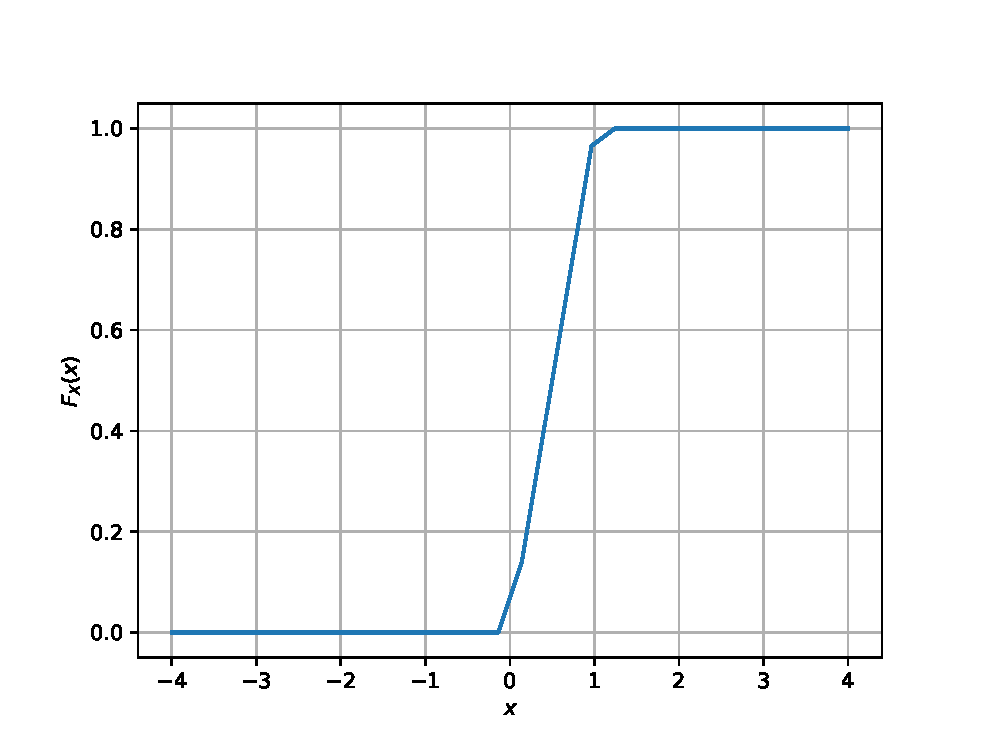
\includegraphics[width=\columnwidth]{figs/1/uni_cdf.eps}
\caption{The CDF of $U$}
\label{fig:uni_cdf}
\end{figure}

%
\item
Find a  theoretical expression for $F_{U}(x)$. \\
\solution
As U is uniform random variable distribution, (between 0 to 1);
$CDF = F_U(x)$
\begin{align}
	F_U(x) = \int_{0}^{x} P_U(x) \,dx 
\end{align}
As uniform distribution, $P_U(x_i) = t$ (t is constant) \\
So,
\begin{align}
	F_U(x) = \int_{0}^{x} t \,dx 
\end{align}
We know that,
\begin{align}
	&F_U(1) = 1 \\
	\implies &\int_{0}^{1} t \,dx = 1 \\
	\implies &t = 1 \\
	\implies &F_U(x) = \int_{0}^{x} 1 \,dx \\
	\implies &F_U(x) = x
\end{align}

\item
The mean of $U$ is defined as
%
\begin{equation}
E\sbrak{U} = \frac{1}{N}\sum_{i=1}^{N}U_i
\end{equation}
%
and its variance as
%
\begin{equation}
\text{var}\sbrak{U} = E\sbrak{U- E\sbrak{U}}^2 
\end{equation}

Write a C program to  find the mean and variance of $U$. \\
\solution
Code file can be found here:
\begin{lstlisting}
	link of c file.
\end{lstlisting}
Mean=0.500007 \\
Variance=0.083301
\item Verify your result theoretically given that
\end{enumerate}
%
\begin{equation}
E\sbrak{U^k} = \int_{-\infty}^{\infty}x^kdF_{U}(x)
\end{equation}
\solution
from question 1.3 \\
\begin{align}
	F_U(x) = x \\
	E\sbrak{U^k} = \int_{-\infty}^{\infty}x^kdx 
\end{align}
for k = 1,
\begin{align}
	E\sbrak{U} &= \int_{-\infty}^{\infty}xdx \\
	 &= \int_{0}^{1}xdx \\
	 &= \frac{1}{2}
\end{align}
for k = 2,
\begin{align}
	E\sbrak{U^2} &= \int_{-\infty}^{\infty}x^2dx \\
	 &= \int_{0}^{1}x^2dx + 0 \\
	 &= \frac{1}{3}
\end{align}
Mean = 0.5 \\
\begin{align}
	var(x) &= E[U^2] - (E\sbrak{U})^2 \\
	 &= \frac{1}{3} - \left(\frac{1}{2}\right)^2 \\
	 &= \frac{1}{3} - \frac{1}{4} \\
	 &= \frac{1}{12} \\
	 var(x) &= 0.083
\end{align}
\section{Central Limit Theorem}
%
\begin{enumerate}[label=\thesection.\arabic*
,ref=\thesection.\theenumi]

%
\item
Generate $10^6$ samples of the random variable
%
\begin{equation}
X = \sum_{i=1}^{12}U_i -6
\end{equation}
%
using a C program, where $U_i, i = 1,2,\dots, 12$ are  a set of independent uniform random variables between 0 and 1
and save in a file called gau.dat \\
\solution 
\begin{lstlisting}
	link of c file
\end{lstlisting}
%
\item
Load gau.dat in python and plot the empirical CDF of $X$ using the samples in gau.dat. What properties does a CDF have?
\\
\solution The CDF of $X$ is plotted in Fig. \ref{fig:gauss_cdf} \\
\begin{lstlisting}
	link of cdf_plot.py file
\end{lstlisting}
\begin{figure}[h]
\centering
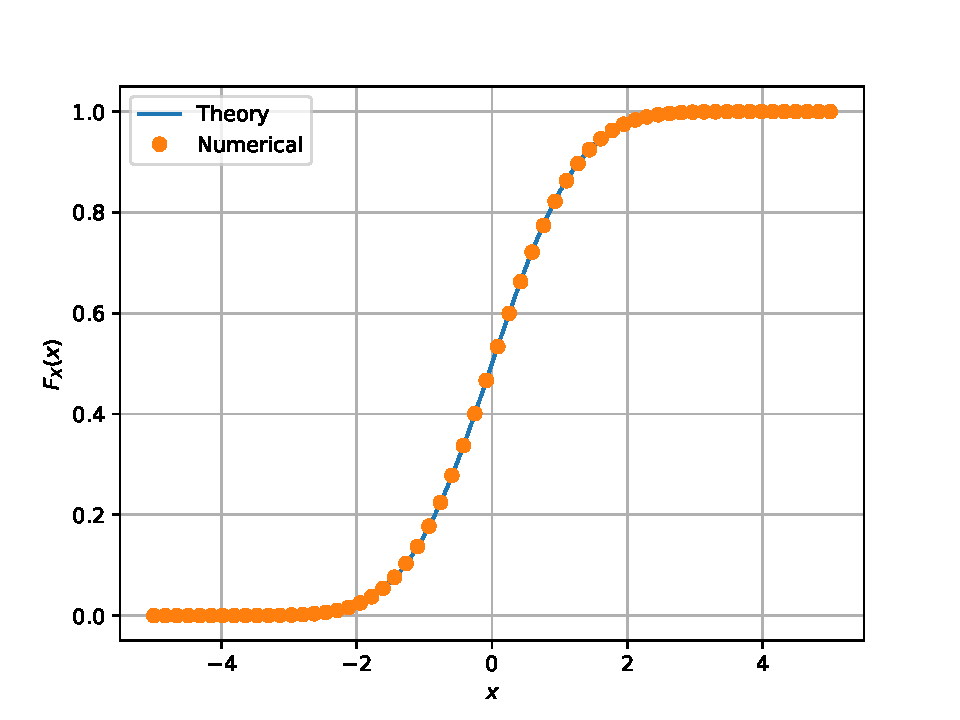
\includegraphics[width=\columnwidth]{figs/2/gau_cdf.pdf}
\caption{The CDF of $X$}
\label{fig:gauss_cdf}
\end{figure}
Properties of CDF:
\begin{itemize}
	\item As x reaches 0 the CDF reaches 0.5 
	\item As x approaches infinity the CDF approaches 1
	\item As x approaches minus infinity the CDF approaches 0 
\end{itemize}
\item
Load gau.dat in python and plot the empirical PDF of $X$ using the samples in gau.dat. The PDF of $X$ is defined as
\begin{align}
p_{X}(x) = \frac{d}{dx}F_{X}(x)
\end{align}
What properties does the PDF have?
\\
\solution The PDF of $X$ is plotted in Fig. \ref{fig:gauss_pdf} using the code below
\begin{lstlisting}
	link of pdf_plot.py
\end{lstlisting}
Proprties of PDF of X:
\begin{itemize}
	\item Graph is simitrical about x=0
	\item Graph have its peak at x=0
\end{itemize}
\begin{figure}[h]
\centering
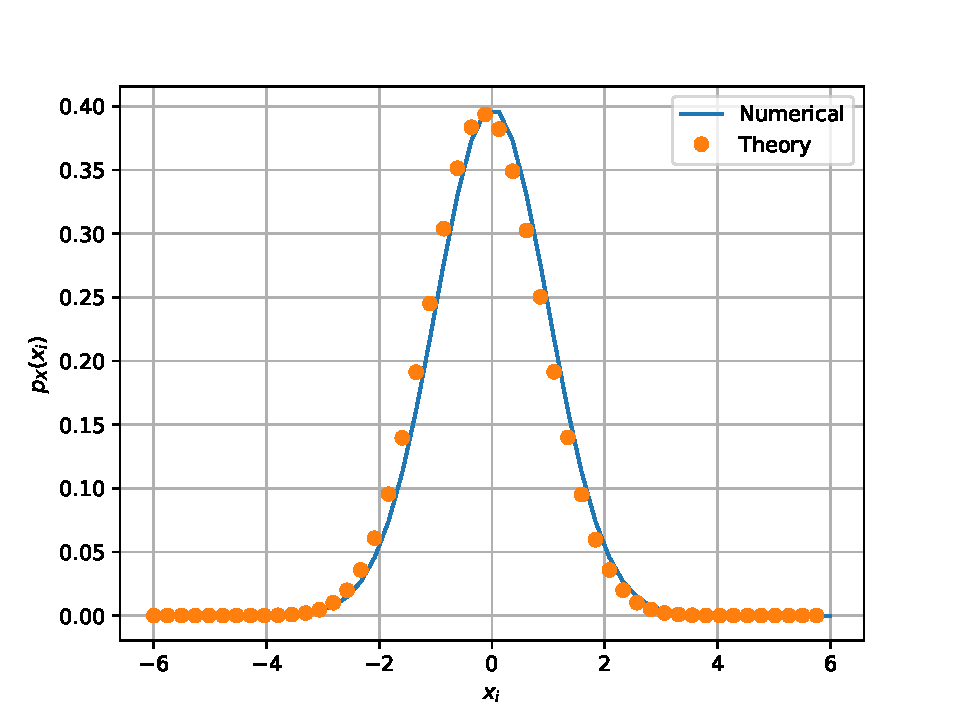
\includegraphics[width=\columnwidth]{figs/2/gauss_pdf.pdf}
\caption{The PDF of $X$}
\label{fig:gauss_pdf}
\end{figure}

\item Find the mean and variance of $X$ by writing a C program. \\
\solution \\
 Mean = 0.000294 \\
 Variance = 0.999560 \\
 c code file can be found at below link:
\begin{lstlisting}
	link of c file
\end{lstlisting}
\item Given that 
\begin{align}
p_{X}(x) = \frac{1}{\sqrt{2\pi}}\exp\brak{-\frac{x^2}{2}}, -\infty < x < \infty,
\end{align}
repeat the above exercise theoretically.
\solution
\begin{align}
	&E[x] = \int_{-\infty}^{\infty} xp_X(x) \,dx \\
	&E[x] = \int_{-\infty}^{\infty} x\frac{1}{\sqrt{2\pi}}\exp\brak{-\frac{x^2}{2}} \,dx \\
	&E[x] = \frac{1}{\sqrt{2\pi}}\int_{-\infty}^{\infty} x\exp\brak{-\frac{x^2}{2}} \,dx \\
	&\frac{x^2}{2} = t \\
	&xdx = dt \\
	&E[x] = \frac{1}{\sqrt{2\pi}} \int_{\infty}^{\infty} \exp(-t) \, dt \\
	&E[x] = 0 \\
	&E[x^2] = \int_{-\infty}^{\infty} x^2p_X(x) \,dx \\
	&E[x^2] = \frac{1}{\sqrt{2\pi}}\int_{-\infty}^{\infty} x^2 \exp\brak{-\frac{x^2}{2}}\,dx \\
	&E[x^2] = \frac{1}{\sqrt{2\pi}}\int_{-\infty}^{\infty} x\left(x \exp\brak{-\frac{x^2}{2}}\right)\,dx \\
\end{align}
Integration by parts,
\begin{align}
	 = x I \,dx - \int I \,dx 
\end{align}
Where $I = \int x \exp\brak{-\frac{x^2}{2}}$ \\
\begin{align}
	\frac{x^2}{2} = t \\
	I = \int \exp(-t) \, dt \\
	I = -\exp(-t) \\
	I = -\exp\brak{-\frac{x^2}{2}} \\
\end{align}
from (2.15),
\begin{align}
	 = -x\exp\brak{-\frac{x^2}{2}} - \int -\exp\brak{-\frac{x^2}{2}} \,dx \\
	 = -x\exp\brak{-\frac{x^2}{2}} + \int \exp\brak{-\frac{x^2}{2}} \,dx 
\end{align}
Substituting limits in (2.13),
\begin{align}
	&E[x^2] = \frac{1}{\sqrt{2\pi}} \int_{-\infty}^{\infty} \exp\brak{-\frac{x^2}{2}} \\
	&E[x^2] = \frac{1}{\sqrt{2\pi}} \times \sqrt{2\pi} \\
	&E[x^2] = 1 \\
	&Var(x) = E[x^2] - \left(E[x]\right)^2 \\
	&Var(x) = 1 - 0 \\
	&Var(x) = 1
\end{align}
\end{enumerate}

\section{From Uniform to Other}
\begin{enumerate}[label=\thesection.\arabic*
,ref=\thesection.\theenumi]
%
\item
Generate samples of 
%
\begin{equation}
V = -2\ln\brak{1-U}
\end{equation}
%
and plot its CDF. \\
\solution 
Code for plot can be found at below link:
\begin{lstlisting}
	link of file
\end{lstlisting}
\begin{figure}[h]
	\centering
	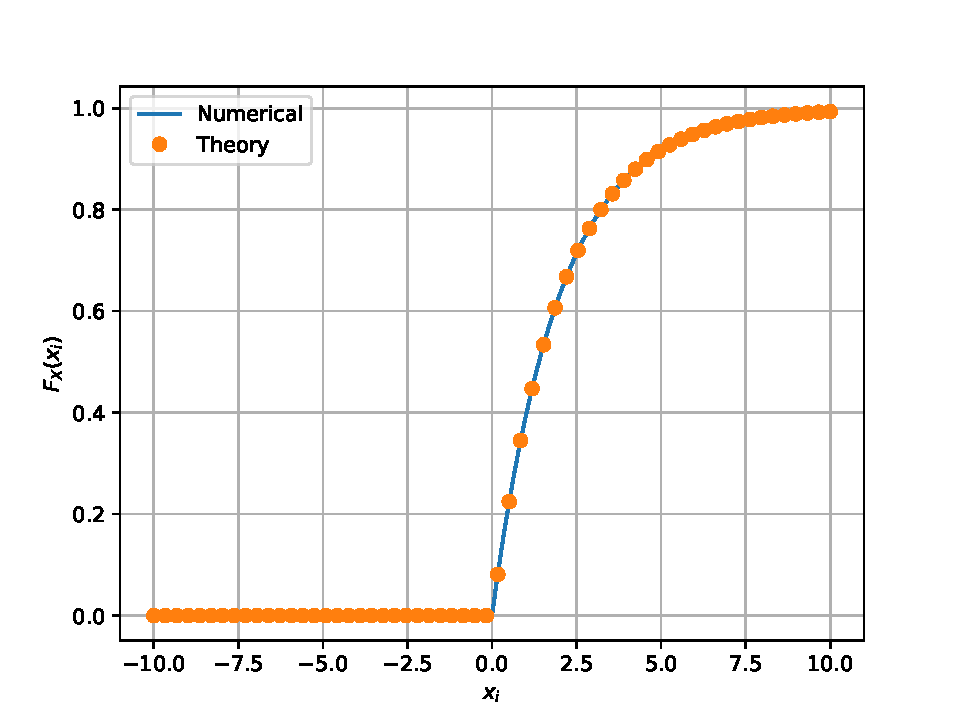
\includegraphics[width=\columnwidth]{figs/3/q3_1.pdf}
	\caption{The CDF of $V$}
	\label{fig:cdf_v}
	\end{figure}
\item Find a theoretical expression for $F_V(x)$. \\
\solution 
\begin{align}
	&F_V(x) = P(V < x) \\
	&F_V(x) = P(-2 \ln(1-U) < x) \\
	&F_V(x) = P\left((1-U) > \exp\brak{-\frac{x}{2}}\right) \\
	&F_V(x) = P\left(U < 1 - \exp\brak{-\frac{x}{2}}\right) \\
	&P(U < x) = x \\
	&P\left(U < 1 - \exp\brak{-\frac{x}{2}}\right) = 1 - \exp\brak{-\frac{x}{2}} \\
	&F_V(x) = 1 - \exp\brak{-\frac{x}{2}}
\end{align}

%
%\item
%Generate the Rayleigh distribution from Uniform. Verify your result through graphical plots.
\end{enumerate}

\section{Triangular Distribution}
\begin{enumerate}[label=\thesection.\arabic*
,ref=\thesection.\theenumi]
%
\item Generate 
	\begin{align}
		T = U_1+U_2
	\end{align}
	\solution 
	T.dat and code files can be found here:
	\begin{lstlisting}
		link of file
	\end{lstlisting}
\item Find the CDF of $T$. \\
\solution

CDF of T, 
\begin{align}
	F_T(t) = P(T<t) \\
	F_T(t) = P(U_1+U_2<t) \\
	0 \leq U_1 \leq 1 \\
	0 \leq U_2 \leq 1 \\
	0 \leq U_1 + U_2 \leq 2 \\
	\forall t>2, P(U_1+U_2<t) = 1 \\
	\forall t<0, P(U_1+U_2<t) = 0 
\end{align}
for $0 \leq t \leq 1$,
% from fig \ref*{}
from fig \ref*{fig:q4_2}
\begin{figure}[h]
	\centering
	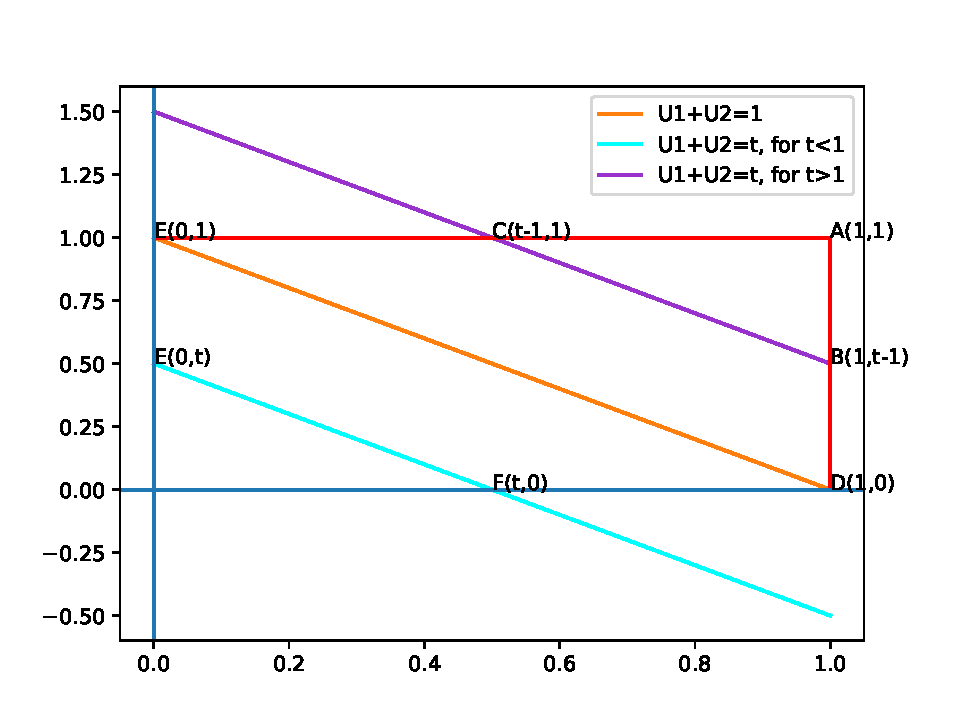
\includegraphics[width=\columnwidth]{figs/4/q4_2.pdf}
	 \caption{q4.2}
	\label{fig:q4_2}    
\end{figure}
Code for plot can be found at below link:
\begin{lstlisting}
	link for plot code 
\end{lstlisting}
\begin{align}
	P(U_1+U_2 <t) &= \frac{\Delta EOF}{\Delta AEOD}\\
	 &= \frac{t^2}{2} \\
\end{align}
for $1 \leq t \leq 2$,
\begin{align}
	P(U_1+U_2 <t) &= \frac{\Delta ABC}{\Delta AEOD}\\
	 &= 1 - \frac{(2-t)^2}{2} 
\end{align}
\begin{align}
	 F_T(t) = 
	 \begin{cases}
		0 & t<0 \\
		\frac{t^2}{2} & 0 \leq t < 1 \\
		1 - \frac{(2-t)^2}{2} & 1 \leq t < 2 \\
		1 & t \geq 2
	 \end{cases}
\end{align}

\item Find the PDF of $T$. \\
\solution 
\begin{align}
	P_T(t) = \frac{d(F_T(t))}{dt} \\
	\therefore P_T(t) = 
	\begin{cases}
		0 & t < 0 \\
		t &  0 \leq t < 1 \\
		2-t & 1 \leq t < 2 \\
		0  & t \geq 2
	\end{cases}
\end{align}
\item Find the theoretical expressions for the PDF and CDF of $T$. \\
\solution 
\begin{align}
	F_T(t) =  
	 \begin{cases}
		0 & t<0 \\
		\frac{t^2}{2} & 0 \therefore \leq t < 1 \\
		1 - \frac{(2-t)^2}{2} & 1 \leq t < 2 \\
		1 & t \geq 2
	 \end{cases} \\
	 P_T(t) = 
	 \begin{cases}
		 0 & t < 0 \\
		 t &  0 \leq t < 1 \\
		 2-t & 1 \leq t < 2 \\
		 0  & t \geq 2
	 \end{cases}
\end{align}
\item Verify your results through a plot. \\
\solution 
Code files for plots can be found at:
\begin{lstlisting}
	link for pdf and cdf plots
\end{lstlisting}
PDF of T: fig \ref*{fig:T_pdf} \\
CDF of T: fig \ref*{fig:T_cdf}
\begin{figure}[h]
	\centering
	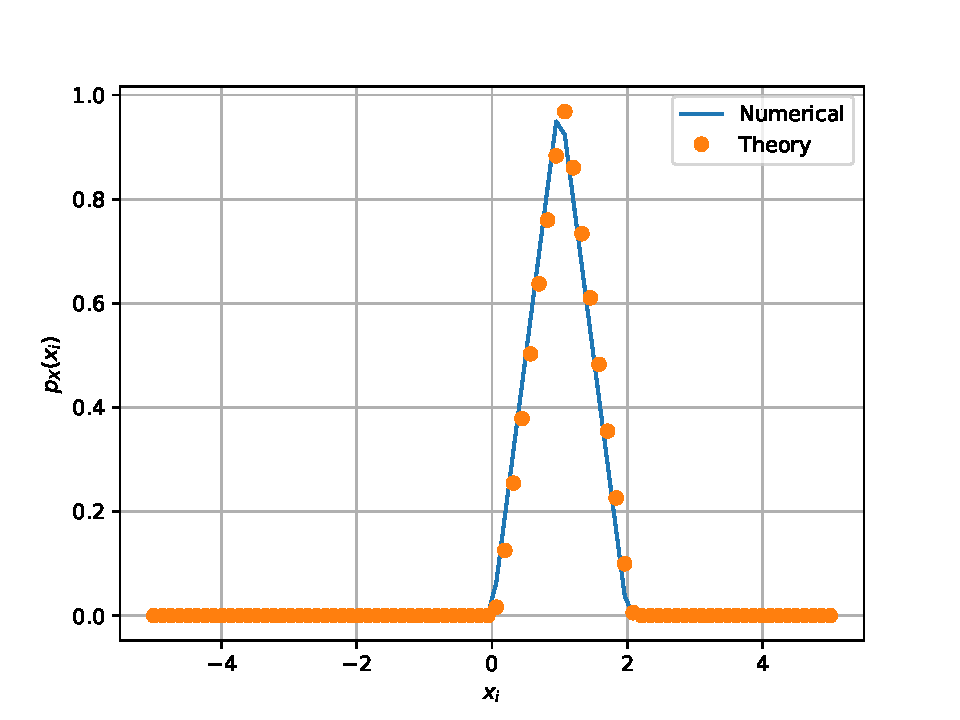
\includegraphics[width=\columnwidth]{figs/4/T_pdf.pdf}
	 \caption{PDF of T}
	\label{fig:T_pdf}
\end{figure}
\begin{figure}[h]
	\centering
	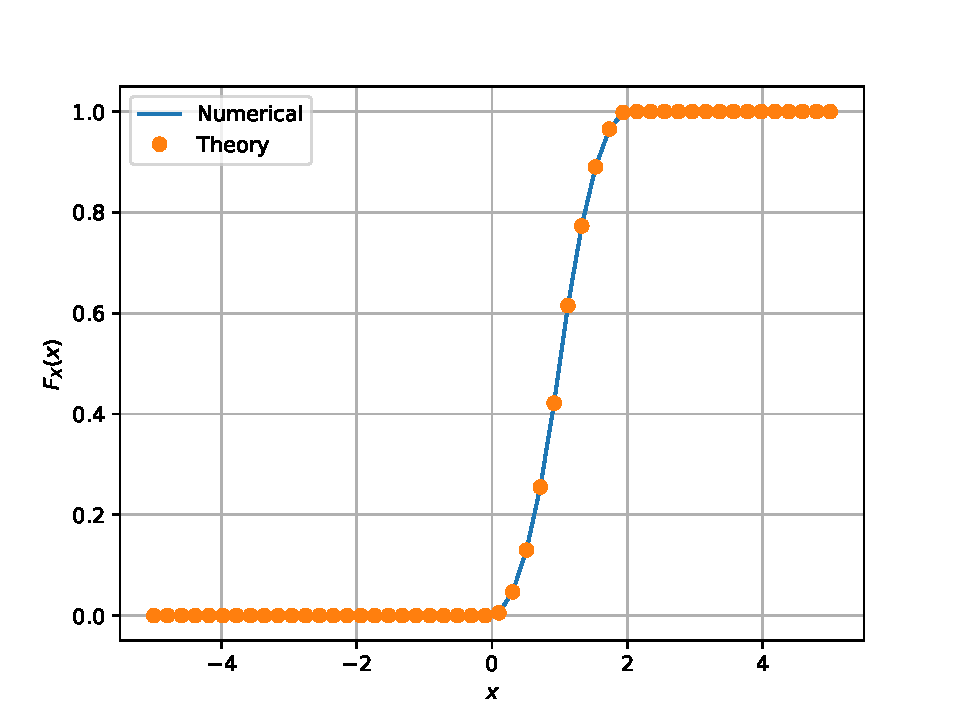
\includegraphics[width=\columnwidth]{figs/4/T_cdf.pdf}
	 \caption{CDF of T}
	\label{fig:T_cdf}
\end{figure}
\end{enumerate}
% \section{Maximul Likelihood}
% \begin{enumerate}[label=\thesection.\arabic*
% ,ref=\thesection.\theenumi]
% \item Generate 
% \begin{equation}
% Y = AX+N,
% \end{equation}
% 		where $A = 5 \text{ dB}, X \i \cbrak{1,-1}$,  is Bernoulli and $N \sim \gauss{0}{1}$.
% 	\item Plot $Y$.
% 	\item Guess how to estimate $X$ from $Y$.
% \item
% \label{ml-ch4_sim}
% Find 
% \begin{equation}
% 	P_{e|0} = \pr{\hat{X} = -1|X=1}
% \end{equation}
% and 
% \begin{equation}
% 	P_{e|1} = \pr{\hat{X} = 1|X=-1}
% \end{equation}
% %
% \item Find $P_e$.

% %
% \item
% Verify by plotting  the theoretical $P_e$.  

% 		\end{enumerate}
% \section{Gaussian to Other}
% \begin{enumerate}[label=\thesection.\arabic*
% ,ref=\thesection.\theenumi]
% \item
% Let $X_1 \sim  \gauss{0}{1}$ and $X_2 \sim  \gauss{0}{1}$. Plot the CDF and PDF of
% %
% \begin{equation}
% V = X_1^2 + X_2^2
% \end{equation}
% %

% %
% %
% \item
% If
% %
% \begin{equation}
% F_{V}(x) = 
% \begin{cases}
% 1 - e^{-\alpha x} & x \geq 0 \\
% 0 & x < 0,
% \end{cases}
% \end{equation}
% %
% find $\alpha$.

% %
% \item
% \label{ch3_raleigh_sim}
% Plot the CDF and PDf of
% %
% \begin{equation}
% A = \sqrt{V}
% \end{equation}
% %


% \end{enumerate}

% \section{Conditional Probability}
% \begin{enumerate}[label=\thesection.\arabic*
% ,ref=\thesection.\theenumi]
% \item
% \item
% \label{ch4_sim}
% Plot 
% \begin{equation}
% P_e = \pr{\hat{X} = -1|X=1}
% \end{equation}
% %
% for 
% \begin{equation}
% Y = AX+N,
% \end{equation}
% where $A$ is Raleigh with $E\sbrak{A^2} = \gamma, N \sim \gauss{0}{1}, X \in \brak{-1,1}$ for $0 \le \gamma \le 10$ dB.

% %
% \item
% Assuming that $N$ is a constant, find an expression for $P_e$.  Call this $P_e(N)$

% %
% \item
% %
% \label{ch4_anal}
% For a function $g$,
% \begin{equation}
% E\sbrak{g(X)} = \int_{-\infty}^{\infty}g(x)p_{X}(x)\, dx
% \end{equation}
% %
% Find $P_e = E\sbrak{P_e(N)}$.

% %
% \item
% Plot $P_e$ in problems \ref{ch4_sim} and \ref{ch4_anal} on the same graph w.r.t $\gamma$.  Comment.

% 		\end{enumerate}
% \section{Two Dimensions}
% Let 
% \begin{equation}
% \mbf{y} = A\mbf{x} + \mbf{n},
% \end{equation}
% where 
% \begin{align}
% x &\in \brak{\mbf{s}_0,\mbf{s}_1}, 
% \mbf{s}_0 = 
% \begin{pmatrix}
% 1 
% \\
% 0
% \end{pmatrix},
% \mbf{s}_1 = 
% \begin{pmatrix}
% 0 
% \\
% 1
% \end{pmatrix}
% \\
% \mbf{n} &= 
% \begin{pmatrix}
% n_1
% \\
% n_2
% \end{pmatrix},
% n_1,n_2 \sim \gauss{0}{1}.
% \end{align}
% %
% \begin{enumerate}[label=\thesection.\arabic*
% ,ref=\thesection.\theenumi]

% %%
% \item
% \label{ch5_fsk}
% Plot 
% %
% \begin{equation}
% \mbf{y}|\mbf{s}_0 \text{ and } \mbf{y}|\mbf{s}_1
% \end{equation}
% %
% on the same graph using a scatter plot.

% %
% \item
% For the above problem, find a decision rule for detecting the symbols $\mbf{s}_0 $ and $\mbf{s}_1$.

% %
% \item
% Plot 
% \begin{equation} 
% P_e = \pr{\hat{\mbf{x}} = \mbf{s}_1|\mbf{x} = \mbf{s}_0}
% \end{equation}
% with respect to the SNR from 0 to 10 dB.

% %
% \item
% Obtain an expression for $P_e$. Verify this by comparing the theory and simulation plots on the same graph.

% %
% 		\end{enumerate}
\end{document}